\documentclass{article}


\usepackage{authblk}
\usepackage[T1]{fontenc}
\usepackage{indentfirst}
\usepackage{graphicx}
\usepackage{caption}
\usepackage{hyperref}

\begin{document}

\title{Optical Tweezer}
\author[a]{Woojin Han}
\affil[a]{Seoul National University, Seoul 151-747, Korea}
\maketitle
\begin{abstract}
    this is abstract
\end{abstract}

\section{Introduction}
\label{sec:intro}
In this experiment, trapping force of gaussian intensity laser to polystyrene bead is measured.
It assumes that linear drag force is applied to the beads obtained by Stoke's law(\ref{intro:Stokes_law})
The assumption allows to calculate trapping force only by measuring critical velocity(\ref{results:tweezing_force}), the velocity when beads fails to captured.
The dynamic viscosity between water and the beads are measurable by detecting Brownian motion(\ref{results:viscosity}), the precise calculation is provided(\ref{intro:Brownian_motion}).
And clever analysis method and its limitation is suggested and performed (\ref{results:modified_brownian_analysis}).
Furthermore, relation between trapping force and refractive index is modelized numerically, refrative index of polystyrene beads is calculated(\ref{discussion:refractive_index_calculation}).


\subsection{Dragging Force : Stoke's Law}
\label{intro:Stokes_law}

In general, drag force have relation to velocity $\vec{F}(\vec{v})=f(v) \hat{v}$.
Taylor expansion of function $f$ simply induces major order by velocity, using condtion of $f(0)=0$, $\vec{F}(\vec{v})=-(bv+cv^2+\mathcal{O}(v^3))\hat{v}$.
Each order of drag force has dependancy with fluid's property, density or viscosity.

\begin{equation}
    f_s(v) = -6 \pi R \eta v
\label{equation:Stokes_law}
\end{equation}

\begin{equation}
    f_q(v) = \frac{1}{2} \rho C_D A v^2
\label{equation:quadratic_drag}
\end{equation}

\begin{equation}
    \frac{f_q}{f_s} = \frac{C_D A}{12 \pi R^2} \frac{R \rho v}{\eta} := \frac{C_D A}{12 \pi R^2} R_e 
\label{equation:reynolds_number}
\end{equation}

Equation \ref{equation:Stokes_law} is Stoke's equation of spherical object, great explaination of linear order drag. $\eta, R$ is dynamic viscosity and radius of object each.
Equation \ref{equation:quadratic_drag} is quadratic drag equation, found by Lord Rayleigh, $\rho, C_D, A$ is density of the fluid, drag coefficient, cross sectional area each.
Equation \ref{equation:reynolds_number} shows the fraction of two different force is proportional to dimensionless Reynolds number($R_e$).
By definition of $R_e$, linear drag force is dominating while Reynolds number is low, and quadratic drag force when high.
In this experiment, order of each parameters is $R \sim 10^{-6} [m], \rho \sim 1000 [kg/m^3], v \sim 10^{-5} [m/s],\eta \sim 10^{-3} [kg / m s]$.
Reynolds number has order of $R_e \sim 10^{-5} \ll 1$.
Therefore, it is absolutely legitimate to claim the drag force follows Stoke's law.(\cite{Reynolds_number})

\subsection{Brownian motion}
\label{intro:Brownian_motion}

Brownian motion is the direct evidnce of the exsistance of atom, enlighted by Einstein.
The theory is induced by calculation of random collision between atom and microparticle.
Since the equation involves randomness, it concerns ensemble mean of the displacement square.

\begin{equation}
    \bar{s^2}= 2Dt =  \frac{2kT}{b} t  = \frac{2kT}{6 \pi R \eta} t
\label{equation:Brownian_motion}
\end{equation}

Equation \ref{equation:Brownian_motion} shows direct relation between mean square displacement and time after a while.
$s, D, k, T, b, t$ is displacement of particle, diffusion constant, Boltzman constant, absolute temperature, linear drag constant and time each.
As you may check the raw experimental results plot on \ref{results:brownian_motion_raw_fig}, it is hard to find a linear relation.
It has two noticable points, firstly the standard of the long time is not well defined.

\begin{equation}
    \bar{s^2} = \frac{2 m k T}{b} (\frac{b}{m}t -1 + e^{-\frac{bt}{m}})
\label{equation:Brownian_motion_Ostein}
\end{equation}

Equation \ref{equation:Brownian_motion_Ostein} helps the first issue, given by Orstein and F{\"u}rth(\cite{Brownian_motion_1}), equivalent with Eientain's result.
The long time $t$ is experimentally considered for $t > 100 \frac{m}{b} \gg \frac{m}{b}$ and the short time limit has checked either. (\ref{results:viscosity}).

Secondary, mathematical foundation of the modified ensemble is given here.
Since Brownian motion is considering randomness, the physical meanings rely on the ensemble average.
It is hard to measure a same particle on same starting position repeatly, the lack of measurement number is inevitable.
Therefore, I assume isotropy of spatial position and construct large ensemble from one trajectory of a particle.
\begin{equation}
    S_\tau = \{ r(\tau)|\sqrt{(x(t+\tau)-x(t))^2+(y(t+\tau)-y(t))^2} \}
    \label{equation:ensemble_construction}
\end{equation}
$S_\tau$ denoted in equation \ref{equation:ensemble_construction} is a definite ensemble of $s$ (absolute value of displacement) in time $\tau$ where $x(t), y(t)$ is the trajectory of one particle.
We need a whole distribution of displacement in time $\tau$ for different starting velocity.
The equation assumes that the particle experiences independantly in every starting position, so the travel of $t$ to $t+\tau$ can be the element of ensemble $S_\tau$.
In experiment, $3000$ frame of particle position is gathered, almost $2000$ elements ensemble can be constructed.
But it has an realistic limitation, for $\tau$ near video running time has too less elements compared to small $\tau$, can not treat both is same linear regression.
The precise application is provided below. (\ref{results:modified_brownian_analysis})


\subsection{Optical tweezer}
\label{intro:optical_tweezer}
While light is reflecting or refracting, the optical force is driven to a refractive matter.
The effects can be calculated in various methods seperated by size of the particle.
For the particles which have smaller size compares to wavelength, Rayleigh scattering(elastic scattering) demonstrates its physics well.
Mie scattering, solves scattering problem of spherical objects analytically, is also a great solution for intermediate size particle. (\cite{T_matrix})
In our experiment, particle size is large enough to neglect the subtle effects of fields, can use ray optical approach.

\begin{figure}[h]
    \centering
    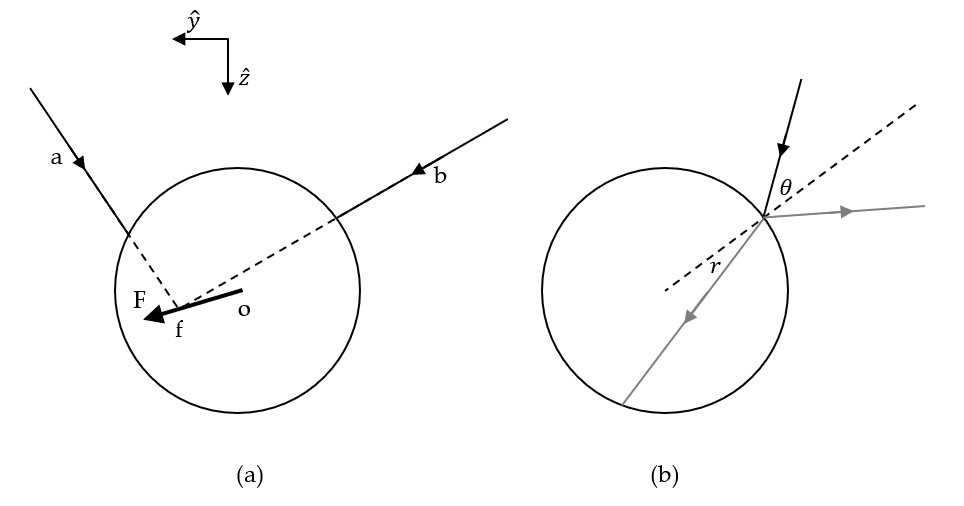
\includegraphics[width=0.8\linewidth]{../results/Optical_tweezer_illust.png}
    \caption{(a) Trap focus $f$ and the forces of dielectric sphere. (b) definition of an angle $\theta$ and $r$ in a single beam scattering}
    \label{Figure:Optical tweezer}
\end{figure}

\begin{equation}
    F_z = \frac{nP}{c} ( 1+ R \cos(2 \theta) - \frac{T^2 [\cos(2 \theta - 2r) + R \cos(2\theta)]}{1+R^2 + 2R \cos 2r} )
    \label{equation:F_z}
\end{equation}

\begin{equation}
    F_y = \frac{nP}{c} (R \sin(2 \theta) - \frac{T^2 [\sin(2 \theta - 2r) + R \sin(2\theta)]}{1+R^2 + 2R \cos 2r} )
    \label{equation:F_y}
\end{equation}
Fig. \ref{Figure:Optical tweezer}(a) illustrates that the direction of trapping force always lies to the trap focus.
We set our z direction parallel to the beam direction, and y direction as trapping focus lies on yz plane.
Equation \ref{equation:F_z} and \ref{equation:F_y} is the force by a single beam, calculated infinite sum of transmitted and reflacted light.(\cite{single_beam})
$n$ is relative refractive index, $P$ is power of the laser, $R$ is reflactance, $T$ is transmittance, $\theta$ is incident angle and $r$ is transmitted angle as Fig. \ref{Figure:Optical tweezer}(b).
I uses Fresnel equation to obtain the reflactance and transmittance of a dielectric object, and follows geometric calculation from \cite{single_beam} to numerically calculate trapping force along y axis.

\begin{figure}[t]
    \centering
    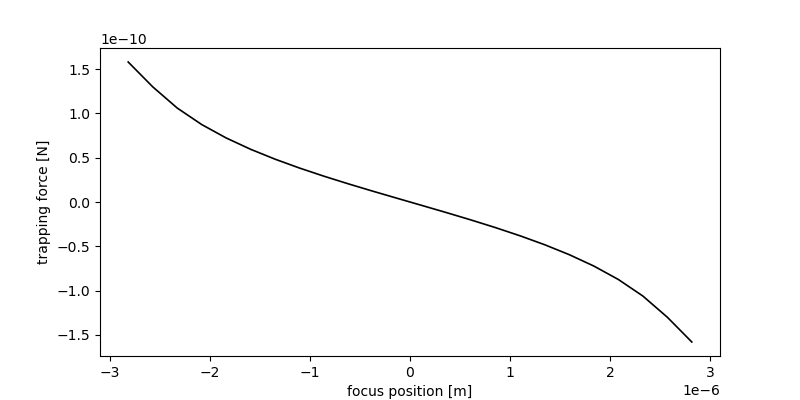
\includegraphics[width=0.8\linewidth]{../results/Optical_tweezer_intro_fig.png}
    \caption{Trapping force - focus position plot in dielectric radius $a = 1\mu m$}
    \label{Figure:Optical tweezer force}
\end{figure}

Fig. \ref{Figure:Optical tweezer force} shows the relation between trapping force and focus position. The force peaks at $0.98a$, very linear under range of $[a,-a]$.
Therefore, it is very valid to assume a trapping force as linear restoring force. I will denote trapping force $F_t = -kx$. The simulation I programmed have two module, get a force by a single beam (\verb|get_force_single_beam|), and get a total gradient force by integrating a beam given in Gaussian intensity (\verb|get_trapping_force|).
I write more details in \ref{discussion:optical_tweezer_simulation}, which whole code is uploaded in \url{https://github.com/WoojinHan24/Optical_Tweezer}

\begin{equation}
    m \ddot{x} =-b\dot{x} -k(x-vt)
    \label{equation:EOM_of_optical_tweezer}
\end{equation}
\begin{equation}
    |x(t) - vt| < a ,    \frac{vb}{k} < a 
    \label{equation:trapping criteria}
\end{equation}

Therefore, we can modelize a particle of mass $m$ and its position $x$ follows an Equation \ref{equation:EOM_of_optical_tweezer}. $v$ stands for velocity of microscope stage, which we measured in the experiments.
Equation \ref{equation:trapping criteria} shows the clear relation between trapping coefficient($k$), we want to measure, and critical velocity($v$), we had measure.


\section{Experiment}

\section{Results}
\subsection{Brownian moiton : viscosity}
\label{results:brownian_motion_raw_fig}
repeated measurement is not sufficient to calculate 'ensemble average'.
The bead, used in experiment, radius is to diverse to assume isotropy between beads.
For example, $2 [\mu m]$ bead contains $2 \pm 0.2 [\mu m]$ which is not negliable to set an ensemble.
\cite{polybead_spec}
\label{results:viscosity}
\label{results:modified_brownian_analysis}
\subsection{Tweezing Force}
\label{results:tweezing_force}

\section{Discussion}


\subsection{optical tweezer model}
\label{discussion:optical_tweezer_simulation}
\subsection{Refractive index}
\label{discussion:refractive_index_calculation}

\bibliography{optical_tweezer_ref}
\bibliographystyle{plain}
\end{document}